\section{eo\-Int\-Above\-Bound Class Reference}
\label{classeo_int_above_bound}\index{eoIntAboveBound@{eoIntAboveBound}}
An eo\-Int\-Bound bounded from above only.  


{\tt \#include $<$eo\-Int\-Bounds.h$>$}

Inheritance diagram for eo\-Int\-Above\-Bound::\begin{figure}[H]
\begin{center}
\leavevmode
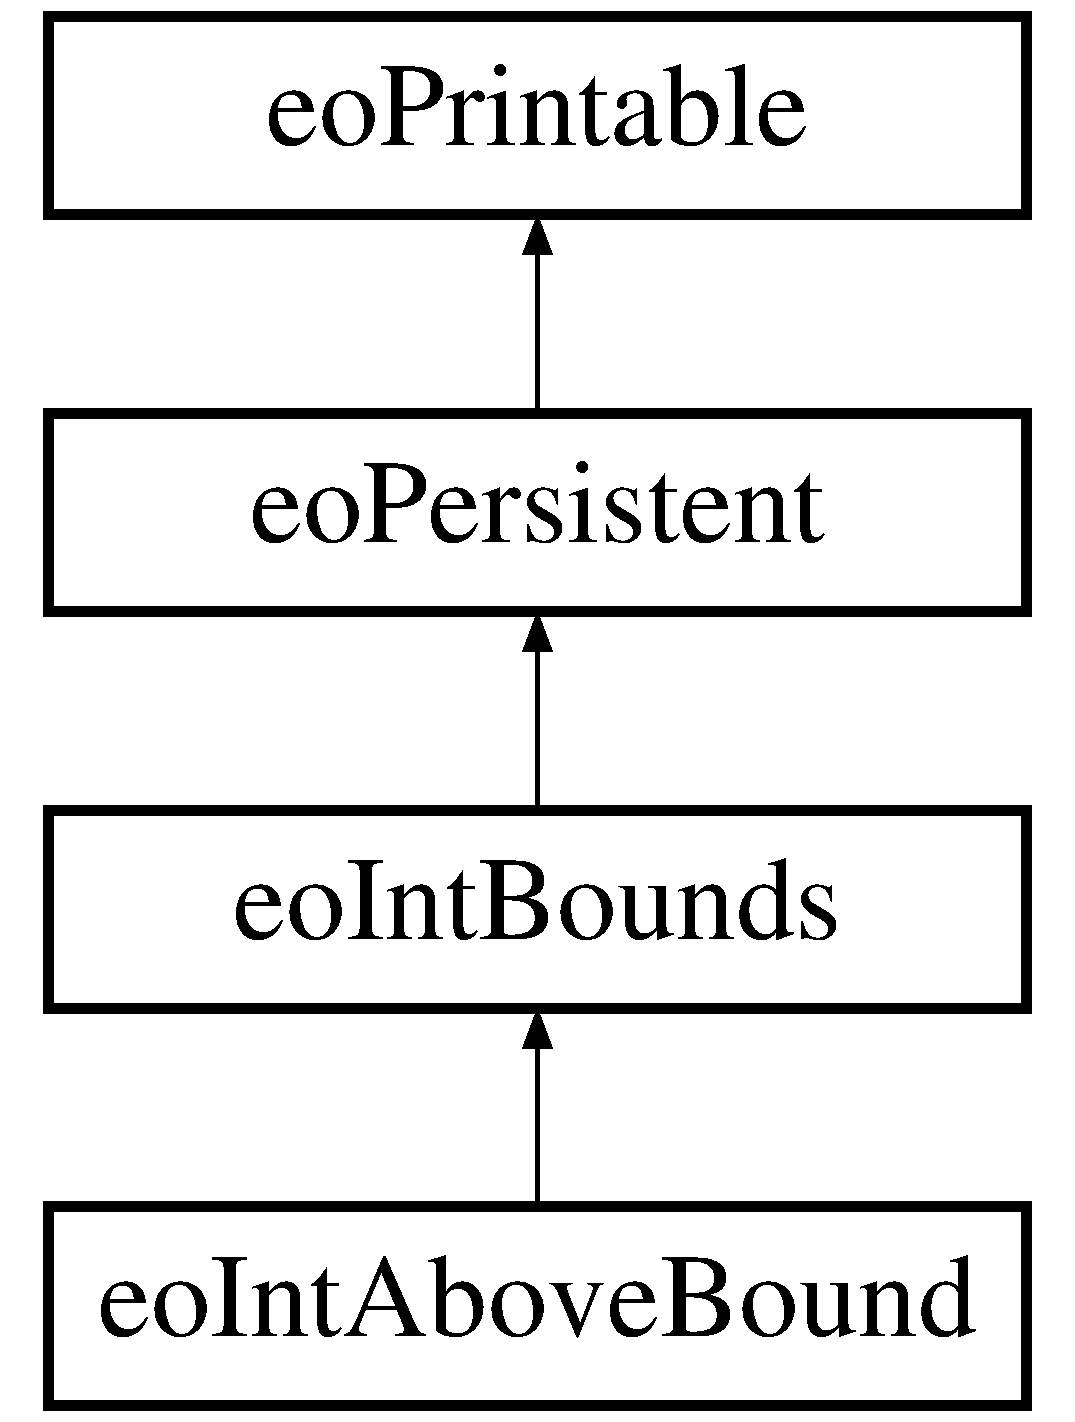
\includegraphics[height=4cm]{classeo_int_above_bound}
\end{center}
\end{figure}
\subsection*{Public Member Functions}
\begin{CompactItemize}
\item 
{\bf eo\-Int\-Above\-Bound} (long int \_\-max=0)\label{classeo_int_above_bound_a1}

\begin{CompactList}\small\item\em Simple bounds = minimum. \item\end{CompactList}\item 
virtual long int {\bf maximum} () const \label{classeo_int_above_bound_a2}

\begin{CompactList}\small\item\em get maximum value ::exception if does not exist \item\end{CompactList}\item 
virtual long int {\bf minimum} () const \label{classeo_int_above_bound_a3}

\begin{CompactList}\small\item\em get minimum value ::exception if does not exist \item\end{CompactList}\item 
virtual long int {\bf range} () const \label{classeo_int_above_bound_a4}

\begin{CompactList}\small\item\em get range ::exception if unbounded \item\end{CompactList}\item 
virtual double {\bf uniform} ({\bf eo\-Rng} \&\_\-rng=eo::rng) const \label{classeo_int_above_bound_a5}

\begin{CompactList}\small\item\em random generator of uniform numbers in bounds uses same naming convention than eo::rng ::exception if unbounded \item\end{CompactList}\item 
virtual long int {\bf random} ({\bf eo\-Rng} \&\_\-rng=eo::rng) const \label{classeo_int_above_bound_a6}

\item 
virtual bool {\bf is\-Bounded} (void) const \label{classeo_int_above_bound_a7}

\begin{CompactList}\small\item\em Self-Test: true if $\ast$$\ast$$\ast$both$\ast$$\ast$$\ast$ a min and a max. \item\end{CompactList}\item 
virtual bool {\bf has\-No\-Bound\-At\-All} (void) const \label{classeo_int_above_bound_a8}

\begin{CompactList}\small\item\em Self-Test: true if no min $\ast$$\ast$$\ast$and$\ast$$\ast$$\ast$ no max hence no further need to test/truncate/fold anything. \item\end{CompactList}\item 
virtual bool {\bf is\-Min\-Bounded} (void) const \label{classeo_int_above_bound_a9}

\begin{CompactList}\small\item\em Self-Test: bounded from below??? \item\end{CompactList}\item 
virtual bool {\bf is\-Max\-Bounded} (void) const \label{classeo_int_above_bound_a10}

\begin{CompactList}\small\item\em Self-Test: bounded from above??? \item\end{CompactList}\item 
virtual bool {\bf is\-In\-Bounds} (double \_\-r) const \label{classeo_int_above_bound_a11}

\begin{CompactList}\small\item\em Test on a value: is it in bounds? \item\end{CompactList}\item 
virtual void {\bf folds\-In\-Bounds} (double \&\_\-r) const \label{classeo_int_above_bound_a12}

\begin{CompactList}\small\item\em Put value back into bounds - by folding back and forth. \item\end{CompactList}\item 
virtual void {\bf truncate} (double \&\_\-r) const \label{classeo_int_above_bound_a13}

\begin{CompactList}\small\item\em Put value back into bounds - by truncating to a boundary value. \item\end{CompactList}\item 
virtual void {\bf read\-From} (std::istream \&\_\-is)
\begin{CompactList}\small\item\em Read object. \item\end{CompactList}\item 
virtual void {\bf print\-On} (std::ostream \&\_\-os) const 
\begin{CompactList}\small\item\em Write object. \item\end{CompactList}\item 
virtual {\bf eo\-Int\-Bounds} $\ast$ {\bf dup} () const \label{classeo_int_above_bound_a16}

\begin{CompactList}\small\item\em for memory managements - ugly \item\end{CompactList}\end{CompactItemize}
\subsection*{Private Attributes}
\begin{CompactItemize}
\item 
long int {\bf rep\-Maximum}\label{classeo_int_above_bound_r0}

\end{CompactItemize}


\subsection{Detailed Description}
An eo\-Int\-Bound bounded from above only. 



Definition at line 441 of file eo\-Int\-Bounds.h.

\subsection{Member Function Documentation}
\index{eoIntAboveBound@{eo\-Int\-Above\-Bound}!readFrom@{readFrom}}
\index{readFrom@{readFrom}!eoIntAboveBound@{eo\-Int\-Above\-Bound}}
\subsubsection{\setlength{\rightskip}{0pt plus 5cm}virtual void eo\-Int\-Above\-Bound::read\-From (std::istream \& {\em \_\-is})\hspace{0.3cm}{\tt  [inline, virtual]}}\label{classeo_int_above_bound_a14}


Read object. 

\begin{Desc}
\item[Parameters:]
\begin{description}
\item[{\em \_\-is}]A std::istream. but reading should not be done here, because of bound problems see eo\-Int\-Vector\-Bounds \end{description}
\end{Desc}


Implements {\bf eo\-Persistent} {\rm (p.\,\pageref{classeo_persistent_a1})}.

Definition at line 512 of file eo\-Int\-Bounds.h.\index{eoIntAboveBound@{eo\-Int\-Above\-Bound}!printOn@{printOn}}
\index{printOn@{printOn}!eoIntAboveBound@{eo\-Int\-Above\-Bound}}
\subsubsection{\setlength{\rightskip}{0pt plus 5cm}virtual void eo\-Int\-Above\-Bound::print\-On (std::ostream \& {\em \_\-os}) const\hspace{0.3cm}{\tt  [inline, virtual]}}\label{classeo_int_above_bound_a15}


Write object. 

It's called print\-On since it prints the object on a stream. \begin{Desc}
\item[Parameters:]
\begin{description}
\item[{\em \_\-os}]A std::ostream. \end{description}
\end{Desc}


Implements {\bf eo\-Printable} {\rm (p.\,\pageref{classeo_printable_a1})}.

Definition at line 521 of file eo\-Int\-Bounds.h.

The documentation for this class was generated from the following file:\begin{CompactItemize}
\item 
eo\-Int\-Bounds.h\end{CompactItemize}
